\clearpage\thispagestyle{empty}\SourceLeaf{002}
\vspace*{1cm}
\begin{center}\small
\textbf{CARL FRIEDRICH GAUSS: WERKE}\\[1em]
\textbf{BAND III.}
\end{center}
\clearpage

\clearpage\thispagestyle{empty}\SourceLeaf{004}
\vspace*{1cm}
\begin{center}\small
\textbf{CARL FRIEDRICH GAUSS}\\[0.5em]
\textbf{WERKE}\\[1em]
\textbf{DRITTER BAND}\\[2em]
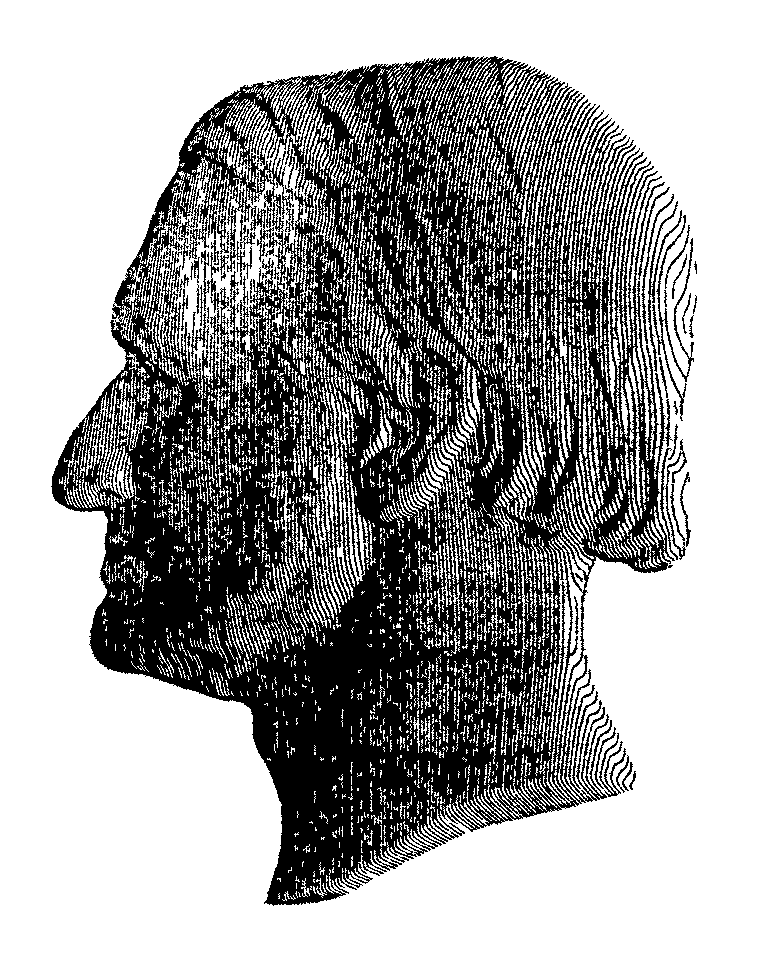
\includegraphics[width=1.65in]{assets/portrait_native004_complete.png}\\[2em]
\textbf{HERAUSGEGEBEN}\\[0.5em]
\textbf{VON DER}\\[0.5em]
\textbf{KÖNIGLICHEN GESELLSCHAFT DER WISSENSCHAFTEN}\\[0.5em]
\textbf{ZU GÖTTINGEN}\\[1em]
\textbf{1866.}
\end{center}
\clearpage

\clearpage\thispagestyle{empty}\SourceLeaf{006}
\vspace*{1cm}
\begin{center}\small
\textbf{EIN NEUER BEWEIS}\\[0.75em]
\textbf{DES SATZES,}\\[0.75em]
\textbf{DASS JEDES POLYNOM}\\[0.5em]
\textbf{}\\[0.75em]
\textbf{IN EINER VARIABLEN}\\[0.75em]
\textbf{IN REELLE FAKTOREN ERSTEN ODER ZWEITEN GRADES}\\[0.75em]
\textbf{ZERLEGT WERDEN KANN}\\[1.5em]
\textbf{ZUR ERLANGUNG}\\[0.5em]
\textbf{DER HÖCHSTEN WÜRDEN IN DER PHILOSOPHIE}\\[0.5em]
\textbf{DER HOCHBERÜHMTEN PHILOSOPHISCHEN FAKULTÄT}\\[0.75em]
\textbf{DER ACADEMIA JULIA CAROLINA}\\[1.5em]
\textbf{VORGELEGT VON}\\[0.75em]
\textbf{CARL FRIEDRICH GAUSS}\\[1.5em]
\rule{0.65\linewidth}{0.4pt}\\[0.75em]
\textbf{HELMSTEDT}\\[0.5em]
\textbf{BEI C. G. FLECKEISEN. MDCCLXXXXIX.}
\end{center}

\clearpage
